\chapter{Konfigurationsraum}

% https://cs.stanford.edu/people/eroberts/courses/soco/projects/1998-99/robotics/definitions.html

Bei einer Roboterlänge und -breite größer als eins können gewisse Punkte im Occupancy Grid nicht erreicht werden, ohne Hindernisse oder Grenzen zu überdecken. 
Aus diesem Grund wird die Roboterbewegung in eine Punktbewegung (\texttt{robot\_width =  robot\_length = 1}) im sogenannten \textit{Konfigurationsraum} transformiert.
Dazu wird jedes Hindernis im Occupancy Grid um die Roboterdimensionen erweitert.

Je nach Rotation ändern sich die überdeckten Koordinaten im Occupancy Grid.
Um den Verbrauch freier Koordinaten um das Hindernis zu minimieren, schlägt XYZ (TODO) vor, die Roboterrotation in diskrete Zustände zu unterteilen. Die Variable \texttt{rotation\_step} gibt als Teiler von $360$° an, um wie viel Grad sich der Roboter pro Bewegungsschritt drehen kann, wodurch sich \texttt{rotations=360/\texttt{rotation\_step}} unterschiedliche Rotationszustände ergeben.
\begin{figure}[H]
	\centering
	\footnotesize
	\centerline{\resizebox{0.6\linewidth}{!}{\input{bilder/rotation-steps_latex.pdf_tex}}}
	\caption{Für \texttt{rotation\_step=45} ergeben sich $(360 \text{\textdegree} \div 45 \text{\textdegree}) = 8$ Rotationszustände.}
\end{figure}

\vspace*{-0.3cm}
Für das Robotermodell wird eine \texttt{robot\_length*robot\_width} Maske erstellt.
Für jeden Rotationszustand wird die Maske mit \texttt{sklearn.rotate()} gedreht sowie ein \textit{erweitertes Occupancy Grids} generiert. Dazu wird jedes Hindernis sowie jede Grenzkoordinate des ursprünglichen Occupancy Grids um die rotierte Maske erweitert.
\vspace*{0.12cm}
\begin{figure}[H]
	\centering
	\footnotesize
	\centerline{\resizebox{0.9\linewidth}{!}{\input{bilder/robot-mask_latex.pdf_tex}}}
	\caption{Erzeugung eines erweiterten Occupancy Grid für eine Rotation um $45$°}
\end{figure}

Der Konfigurationsraum \texttt{configuration-space[rotation][y][x]} mit den Dimensionen fasst die Erweiterten Occupancy Grids in der Dimension \texttt{[rotation]} zusammen:
\begin{itemize}
\item \texttt{(rotation + 1) \% rotations} $\widehat{=}$ Rotation um \texttt{rotation\_step} gegen den Uhrzeigersinn
\item \texttt{(rotation - 1) \% rotations} $\widehat{=}$ Rotation um \texttt{rotation\_step} im Uhrzeigersinn
\end{itemize}
\vspace*{0.4cm}
\begin{figure}[H]
	\centering
	\footnotesize
	\centerline{\resizebox{1\linewidth}{!}{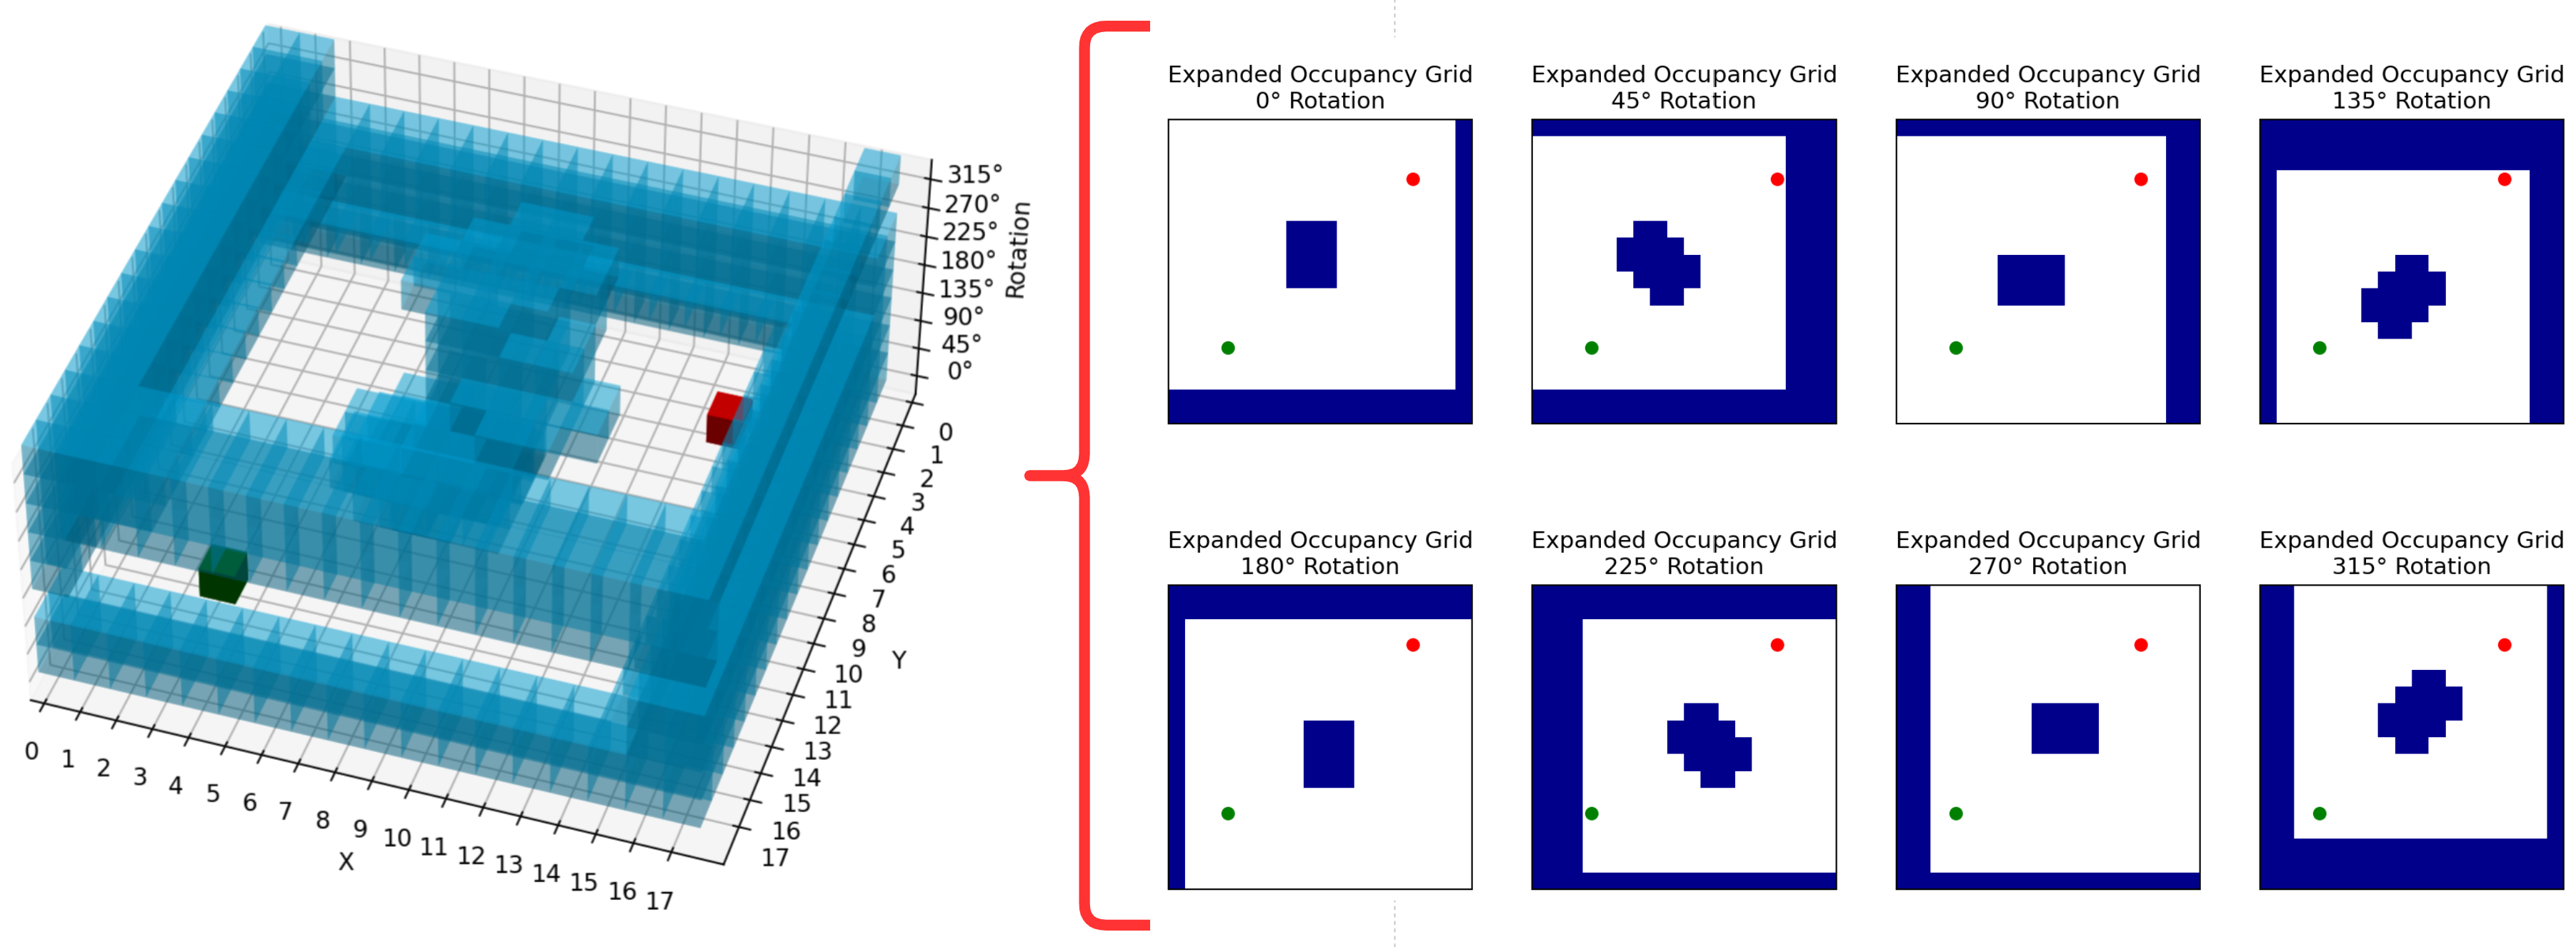
\includegraphics{bilder/configuration-space.png}}}
	\caption{Die erweiterten Occupancy Grids bilden den Konfigurationsraum}
\end{figure}

Der Konfigurationsraum $\texttt{rotations*occupancy\_grid\_length*occupancy\_grid\_width}$ nach XYZ (TODO!) ermöglicht über die Punktbewegung im dreidimensionalen Raum eine kollisionsfreie Translation und Rotation im Occupancy Grid bei minimalem Verbrauch freier Koordinaten. 
Die Position \texttt{x,y} des Roboters sowie dessen Rotationszustand \texttt{rotation} im Occupancy Grid wird dabei im Konfigurationsraum über die Dimensionen \texttt{rotation, y, x} referenziert.


